\documentclass[../rapport_MVEX01-11-05]{subfiles}
\begin{document}
\section{Våra gester}
Handgester kan delas in i två kategorier, statiska och dynamiska. De
statiska gesterna är sådana där handen inte rör sig, utan en enda
bildruta är tillräcklig för att bestämma vad det är för gest. Exempel på
sådana är freds- och segergesten med två fingrar i ett V och ''tumme
upp''-gesten. Dynamiska gester å andra sidan är sådana som innefattar en
rörelse, exempelvis en vinkning. Dessa är betydligt svårare att
behandla ur ett igenkänningsperspektiv, då de kräver en följd av
bildrutor och bilderna därför inte kan behandlas separat.

\begin{figure}[tb]
	\centering 
	\subfloat[A]{
		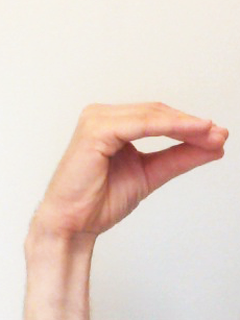
\includegraphics[height=2.5cm]{bilder/gest1.png}
		\label{fig:gester:A}
	}
	% ev. spacing
	\subfloat[B]{
		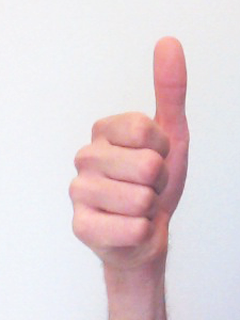
\includegraphics[height=2.5cm]{bilder/gest2.png}
		\label{fig:gester:B}
	}
	% ev. spacing
	\subfloat[C]{
		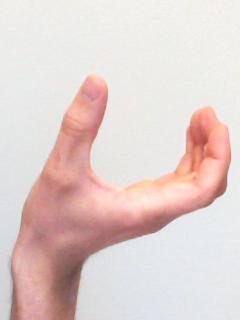
\includegraphics[height=2.5cm]{bilder/gest3.png}
		\label{fig:gester:C}
	}
	% ev. spacing
	\subfloat[D]{
		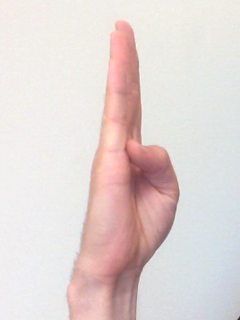
\includegraphics[height=2.5cm]{bilder/gest4.png}
		\label{fig:gester:D}
	}
	% ev. spacing
	\subfloat[E]{
		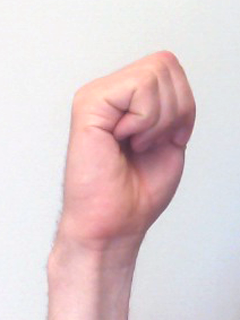
\includegraphics[height=2.5cm]{bilder/gest5.png}
		\label{fig:gester:E}
	}
	\\
	% ev. spacing
	\subfloat[Sten]{
		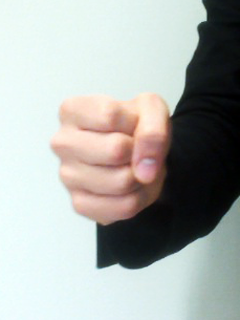
\includegraphics[height=2.5cm]{bilder/gest6.png}
		\label{fig:gester:sten}
	}
	% ev. spacing
	\subfloat[Sax]{
		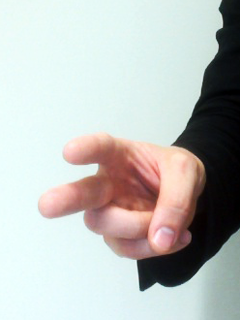
\includegraphics[height=2.5cm]{bilder/gest7.png}
		\label{fig:gester:sax}
	}
	% ev. spacing
	\subfloat[Påse]{
		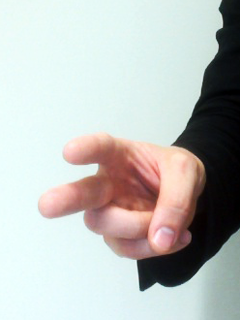
\includegraphics[height=2.5cm]{bilder/gest8.png}
		\label{fig:gester:pase}
	}
	% ev. spacing
	\subfloat[Spock]{
		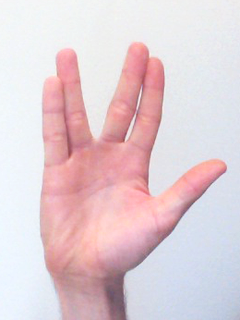
\includegraphics[height=2.5cm]{bilder/gest9.png}
		\label{fig:gester:spock}
	}
	% ev. spacing
	\subfloat[Seger]{
		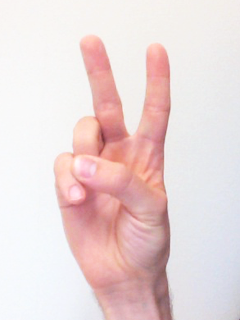
\includegraphics[height=2.5cm]{bilder/gest10.png}
		\label{fig:gester:seger}
	}
	% ev. spacing
	\caption{Vi har tio olika statiska handgester att matcha mot indata.}
	\label{fig:gester}
\end{figure}

Vid testerna av vårt program har vi använt tio statiska gester (figur
\ref{fig:gester}):

\begin{itemize}
 	\item Svenska handalfabetets tecken för A. 4 fingrar hålls ihop och tummen
  möter pekfingret. Hålet mellan tumme och pekfinger är ovalt.

  \item Svenska handalfabetets tecken för B. Sträckt tumme uppåt, i övrigt knutna fingrar, ''tumme upp''.

  \item Svenska handalfabetets tecken för C. Kupad hand med tummen upp från handflatan. Handflatan uppåt
  och lillfingret närmast bröstet. 

  \item Svenska handalfabetets tecken för D. Handen sträckt uppåt med pekfingret mot bröstet. Tummen böjd
  in i handen.

  \item Svenska handalfabetets tecken för E. Knuten hand runt tummen. Pekfingret närmast kroppen. 

  \item Stenen i den traditionella leken ''sten, sax, påse''. Knuten hand, tummen utanför pekfingret. Tummen uppåt.

  \item Saxen i den traditionella leken ''sten, sax, påse''. Pek- och långfinger sträckta framåt, separerade, övriga
  fingrar knutna.

  \item Påsen i den traditionella leken ''sten, sax, påse''. Handen sträckt, fingrarna pekandes framåt.

  \item Spock-hälsning. Handflatan mot kameran, fingrarna sträckta med pek- och
  långfinger ihop, ring- och lillfinger ihop och mellanrum mellan
  lång- och ringfinger. Även kallad Vulcan Salute, från TV-serien Star
  Trek, inspirerad av en judisk hälsning.

  \item Segertecken. Handflatan mot kameran, pek- och långfinger sträckta i
  ett V, övriga fingrar knutna. Kan även ses som en fredssymbol,
  flitigt använd av allierade och motståndsrörelser i de ockuperade
  länderna under andra världskriget.
\end{itemize}

\end{document}
